\documentclass{beamer}

% Pakiety
\usepackage{amsmath, amssymb, graphicx, hyperref}
\usepackage[polish]{babel}
\usepackage{xcolor}
\usepackage[T1]{fontenc}

% Tytuł prezentacji
\title{Importance Sampling}
\author{Natalia Bednarz, Aleksandra Bieniek, Max Stróżyk}
\date{21.01.2025 r.}

\begin{document}

% Strona tytułowa
\begin{frame}
    \titlepage
\end{frame}

% Wprowadzenie
\begin{frame}{Wprowadzenie do IS}
    \textbf{Importance Sampling (IS)} to zaawansowana technika symulacyjna używana do estymacji rzadkich zdarzeń.
    
    \vspace{0.5cm}
    \textbf{Cel:} 
    \begin{itemize}
        \item Klasyczna metoda Monte Carlo (MC) wymaga ogromnej liczby prób do precyzyjnego oszacowania prawdopodobieństwa zdarzeń rzadkich.
        \item IS zmniejsza liczbę prób potrzebnych do osiągnięcia tego samego poziomu dokładności.
    \end{itemize}
\end{frame}

% Idea Importance Sampling
\begin{frame}{Na czym polega Importance Sampling?}
    Główna idea IS polega na:
    \begin{enumerate}
        \item Zmianie rozkładu prawdopodobieństwa zmiennej losowej $X$ na tzw. \textit{rozklad biasing} $f^*(x)$.
        \item Ważeniu wyników próbek z rozkładu $f^*(x)$ poprzez funkcję wagową $W(x)$:
        \[
        W(x) = \frac{f(x)}{f^*(x)},
        \]
        gdzie $f(x)$ to oryginalny rozkład zmiennej losowej.
    \end{enumerate}

    \vspace{0.5cm}
    \textbf{Szacowanie:}
    Prawdopodobieństwo zdarzenia $P(X \geq t)$ w IS oblicza się jako:
    \[
    P(X \geq t) = \mathbb{E}^*\big[W(X) \cdot \mathbb{I}(X \geq t)\big],
    \]
    gdzie $\mathbb{E}^*$ oznacza wartość oczekiwaną względem rozkładu $f^*(x)$.
\end{frame}

% Dlaczego IS działa?
\begin{frame}
    \textbf{Zalety IS:}
    \begin{itemize}
        \item Skupia symulacje na \textit{ważnych} regionach, gdzie zdarzenia rzadkie mają miejsce.
        \item Zmniejsza wariancję estymatora w porównaniu do klasycznej metody MC.
        \item Wykorzystuje \textbf{rozklad biasing}, który zwiększa częstość występowania rzadkich zdarzeń.
    \end{itemize}

    \vspace{0.5cm}
    \textbf{Przykład:}
    \begin{itemize}
        \item Klasyczne MC: Tylko kilka próbek spełnia warunek $X \geq t$, co prowadzi do dużej wariancji.
        \item IS: Dzięki odpowiednio dobranemu $f^*(x)$, większość próbek spełnia warunek $X \geq t$.
    \end{itemize}
\end{frame}

% Wzory IS
\begin{frame}
    \textbf{Ogólna definicja IS:}
    \[
    \mathbb{E}[g(X)] = \int g(x)f(x)dx = \int g(x)W(x)f^*(x)dx = \mathbb{E}^*[g(X)W(X)],
    \]
    gdzie:
    \begin{itemize}
        \item $g(X)$ to funkcja zmiennej losowej, której wartość oczekiwaną estymujemy,
        \item $f(x)$ to oryginalny rozkład prawdopodobieństwa,
        \item $f^*(x)$ to rozkład biasing,
        \item $W(x) = \frac{f(x)}{f^*(x)}$ to funkcja wagowa.
    \end{itemize}

    \vspace{0.5cm}
    \textbf{Wariancja estymatora IS:}
    \[
    \text{Var}^*[g(X)W(X)] = \mathbb{E}^*[g^2(X)W^2(X)] - \left(\mathbb{E}^*[g(X)W(X)]\right)^2.
    \]
\end{frame}

% Przykład zastosowania IS
% \begin{frame}{Przykład zastosowania IS}
%     \textbf{Problem:} Estymacja prawdopodobieństwa $P(X \geq t)$ dla zmiennej losowej $X \sim N(0,1)$ (rozkład normalny).

%     \vspace{0.5cm}
%     \textbf{Metoda MC:}
%     \begin{itemize}
%         \item Generujemy próbki z rozkładu $N(0,1)$.
%         \item Liczymy proporcję próbek spełniających warunek $X \geq t$.
%     \end{itemize}

%     \vspace{0.5cm}
%     \textbf{Metoda IS:}
%     \begin{itemize}
%         \item Wybieramy rozkład biasing $f^*(x) = N(c,1)$, gdzie $c > t$.
%         \item Ważymy próbki funkcją wagową $W(x) = e^{-\frac{c^2}{2}} e^{cX}$.
%     \end{itemize}

%     \vspace{0.5cm}
%     \textbf{Porównanie:}
%     IS znacząco redukuje liczbę próbek potrzebnych do uzyskania niskiej wariancji estymatora.
% \end{frame} 


% Slajd wprowadzający
\begin{frame}{Techniki zmiany rozkładów}
    \vspace{0.5cm}
    \textbf{Scaling} i \textbf{Translation} to dwie podstawowe techniki zmiany rozkładów:
    \begin{itemize}
        \item \textbf{Scaling:} Zmiana skali zmiennej losowej w celu skoncentrowania masy prawdopodobieństwa w interesującym nas regionie.
        \item \textbf{Translation:} Przesunięcie rozkładu w celu zwiększenia liczby próbek w regionie rzadkich zdarzeń.
    \end{itemize}
\end{frame}

% Scaling - definicja i szczegóły matematyczne
\begin{frame}{Scaling}
    \textbf{Scaling} polega na zastosowaniu zmiennej losowej $X$ i przeskalowaniu jej przez współczynnik $a > 1$:
    \[
    X^* = aX.
    \]

    \textbf{Rozkład biasing:}
    \[
    f^*(x) = \frac{1}{a}f\left(\frac{x}{a}\right),
    \]
    gdzie $f(x)$ to oryginalny rozkład zmiennej $X$.

    \vspace{0.5cm}
    \textbf{Ważenie:} Funkcja wagowa $W(x)$ to stosunek gęstości:
    \[
    W(x) = \frac{f(x)}{f^*(x)} = \frac{af(x)}{f(\frac{x}{a})}
    \]
\end{frame}

% Scaling - przykład
\begin{frame}{Scaling - przykład: rozkład Weibulla}
    Rozważmy zmienną losową $X$ z rozkładem Weibulla:
    \[
    f(x) = \frac{b}{\lambda}\left(\frac{x}{\lambda}\right)^{b-1} e^{-(x/\lambda)^b}, \quad x \geq 0.
    \]

    \textbf{Rozkład biasing po skalowaniu:}
    \[
    f^*(x) = \frac{b}{a\lambda}\left(\frac{x}{a\lambda}\right)^{b-1} e^{-\left(\frac{x}{a\lambda}\right)^b}.
    \]

    \textbf{Funkcja wagowa:}
    \[
    W(x) = a^be^{-(1-a^{-b})(\frac{x}{\lambda})^b}
    \]
\end{frame}

% Translation - definicja i szczegóły matematyczne
\begin{frame}{Translation}
    \textbf{Translation} polega na przesunięciu zmiennej losowej $X$ \\ o wartość $c$:
    \[
    X^* = X + c, \quad c > 0.
    \]

    \textbf{Rozkład biasing:}
    \[
    f^*(x) = f(x - c),
    \]
    gdzie $f(x)$ to oryginalny rozkład zmiennej $X$.

    \vspace{0.5cm}
    \textbf{Ważenie:} Funkcja wagowa $W(x)$ to stosunek gęstości:
    \[
    W(x) = \frac{f(x)}{f^*(x)} = \frac{f(x)}{f(x - c)}.
    \]
\end{frame}

% Translation - przykład
\begin{frame}{Translation - przykład: rozkład Gaussa}
    Rozważmy zmienną losową $X$ z rozkładem normalnym $N(0, 1)$:
    \[
    f(x) = \frac{1}{\sqrt{2\pi}} e^{-\frac{x^2}{2}}.
    \]

    \textbf{Rozkład biasing po translacji:}
    \[
    f^*(x) = \frac{1}{\sqrt{2\pi}} e^{-\frac{(x - c)^2}{2}}, \quad c > 0.
    \]

    \textbf{Funkcja wagowa:}
    \[
    W(x) = e^{-\frac{c(2x - c)}{2}}.
    \]
\end{frame}

% Porównanie Scaling i Translation
\begin{frame}{Porównanie Scaling i Translation}
    \begin{itemize}
        \item \textbf{Scaling:}
        \begin{itemize}
            \item Skuteczny dla zmiennych jednorodnych, np. rozkład Weibulla.
            \item Może powodować rozpraszanie masy prawdopodobieństwa w niepożądanych regionach.
        \end{itemize}
        \item \textbf{Translation:}
        \begin{itemize}
            \item Skuteczniejszy w przypadku rozkładów symetrycznych, np. Gaussa.
            \item Nie występuje "efekt wymiarowości" \space jak w skalowaniu.
        \end{itemize}
    \end{itemize}
\end{frame}

% Wprowadzenie do Exponential Twisting
\begin{frame}{Exponential Twisting}
    \textbf{Exponential Twisting (ET)} to zaawansowana technika w importance sampling, polegająca na:
    \begin{itemize}
        \item zmianie rozkładu zmiennej losowej $X$ poprzez "skręcenie"\space jej gęstości,
        \item użyciu rozkładu z modyfikowaną funkcją momentów.
    \end{itemize}

    \vspace{0.5cm}
    \textbf{Cel:} 
    \begin{itemize}
        \item ET minimalizuje wariancję estymatora dzięki optymalnemu \textit{przekierowaniu masy prawdopodobieństwa} w regiony istotnych zdarzeń.
        \item Jest szczególnie skuteczna przy estymacji zdarzeń rzadkich, gdzie klasyczne podejścia mogą zawieść.
    \end{itemize}
\end{frame}

% Idea matematyczna
\begin{frame}
    \textbf{Twisting gęstości:} Nowa gęstość $f^*(x)$ jest generowana przez skręcenie oryginalnej gęstości $f(x)$:
    \[
    f^*(x) = \frac{e^{sx} f(x)}{M(s)},
    \]
    gdzie:
    \begin{itemize}
        \item $M(s) = \mathbb{E}[e^{sX}]$ to funkcja momentów,
        \item $s > 0$ to parametr \textit{skręcenia}, optymalizowany w celu minimalizacji wariancji estymatora.
    \end{itemize}

    \vspace{0.5cm}
    \textbf{Ważenie:} Funkcja wagowa $W(x)$ dla próbki $x$:
    \[
    W(x) = \frac{f(x)}{f^*(x)} = e^{-sx + \mu(s)},
    \]
    gdzie $\mu(s) = \log M(s)$.
\end{frame}

% Optymalny parametr s
\begin{frame}{Parametr $s$}
    Parametr $s$ jest wybierany w celu minimalizacji wariancji \\ estymatora IS. 

    \vspace{0.5cm}
    \textbf{Warunek optymalności:}
    \[
    \mu'(s) = t,
    \]
    gdzie $t$ to wartość progowa zdarzenia rzadkiego (np. $P(X \geq t)$).

    \vspace{0.5cm}
    \textbf{Interpretacja:} Optymalny parametr $s$ \textit{przekierowuje masę prawdopodobieństwa} w kierunku interesującego nas regionu (np. ogona rozkładu).
\end{frame}

% Przykład - Rozkład normalny
\begin{frame}{Przykład: Rozkład Gaussa}
    Rozważmy zmienną losową $X \sim N(0, 1)$. Funkcja momentów:
    \[
    M(s) = \exp\left(\frac{s^2}{2}\right).
    \]

    \textbf{Twisted density:}
    \[
    f^*(x) = \frac{e^{sx} f(x)}{M(s)} = \frac{1}{\sqrt{2\pi}} e^{-\frac{(x - s)^2}{2}}.
    \]

    \textbf{Ważenie:}
    \[
    W(x) = e^{-sx + \frac{s^2}{2}}.
    \]
\end{frame}

% Zalety Exponential Twisting
\begin{frame}{Zalety Exponential Twisting}
    \begin{itemize}
        \item \textbf{Efektywność:} Minimalizuje wariancję estymatora IS.
        \item \textbf{Elastyczność:} Może być stosowana do wielu rozkładów, w tym normalnego, gamma i innych.
        \item Oparta na funkcjach momentów, które są dobrze znane dla wielu standardowych rozkładów.
    \end{itemize}
\end{frame}
\begin{frame}
    \Huge
    \centering
    \textbf{\textcolor{red}{TESTOWANIE NUMERYCZNE}}
\end{frame}



\begin{frame}{Testowanie numeryczne}{Rozkład Normalny}\begin{figure} 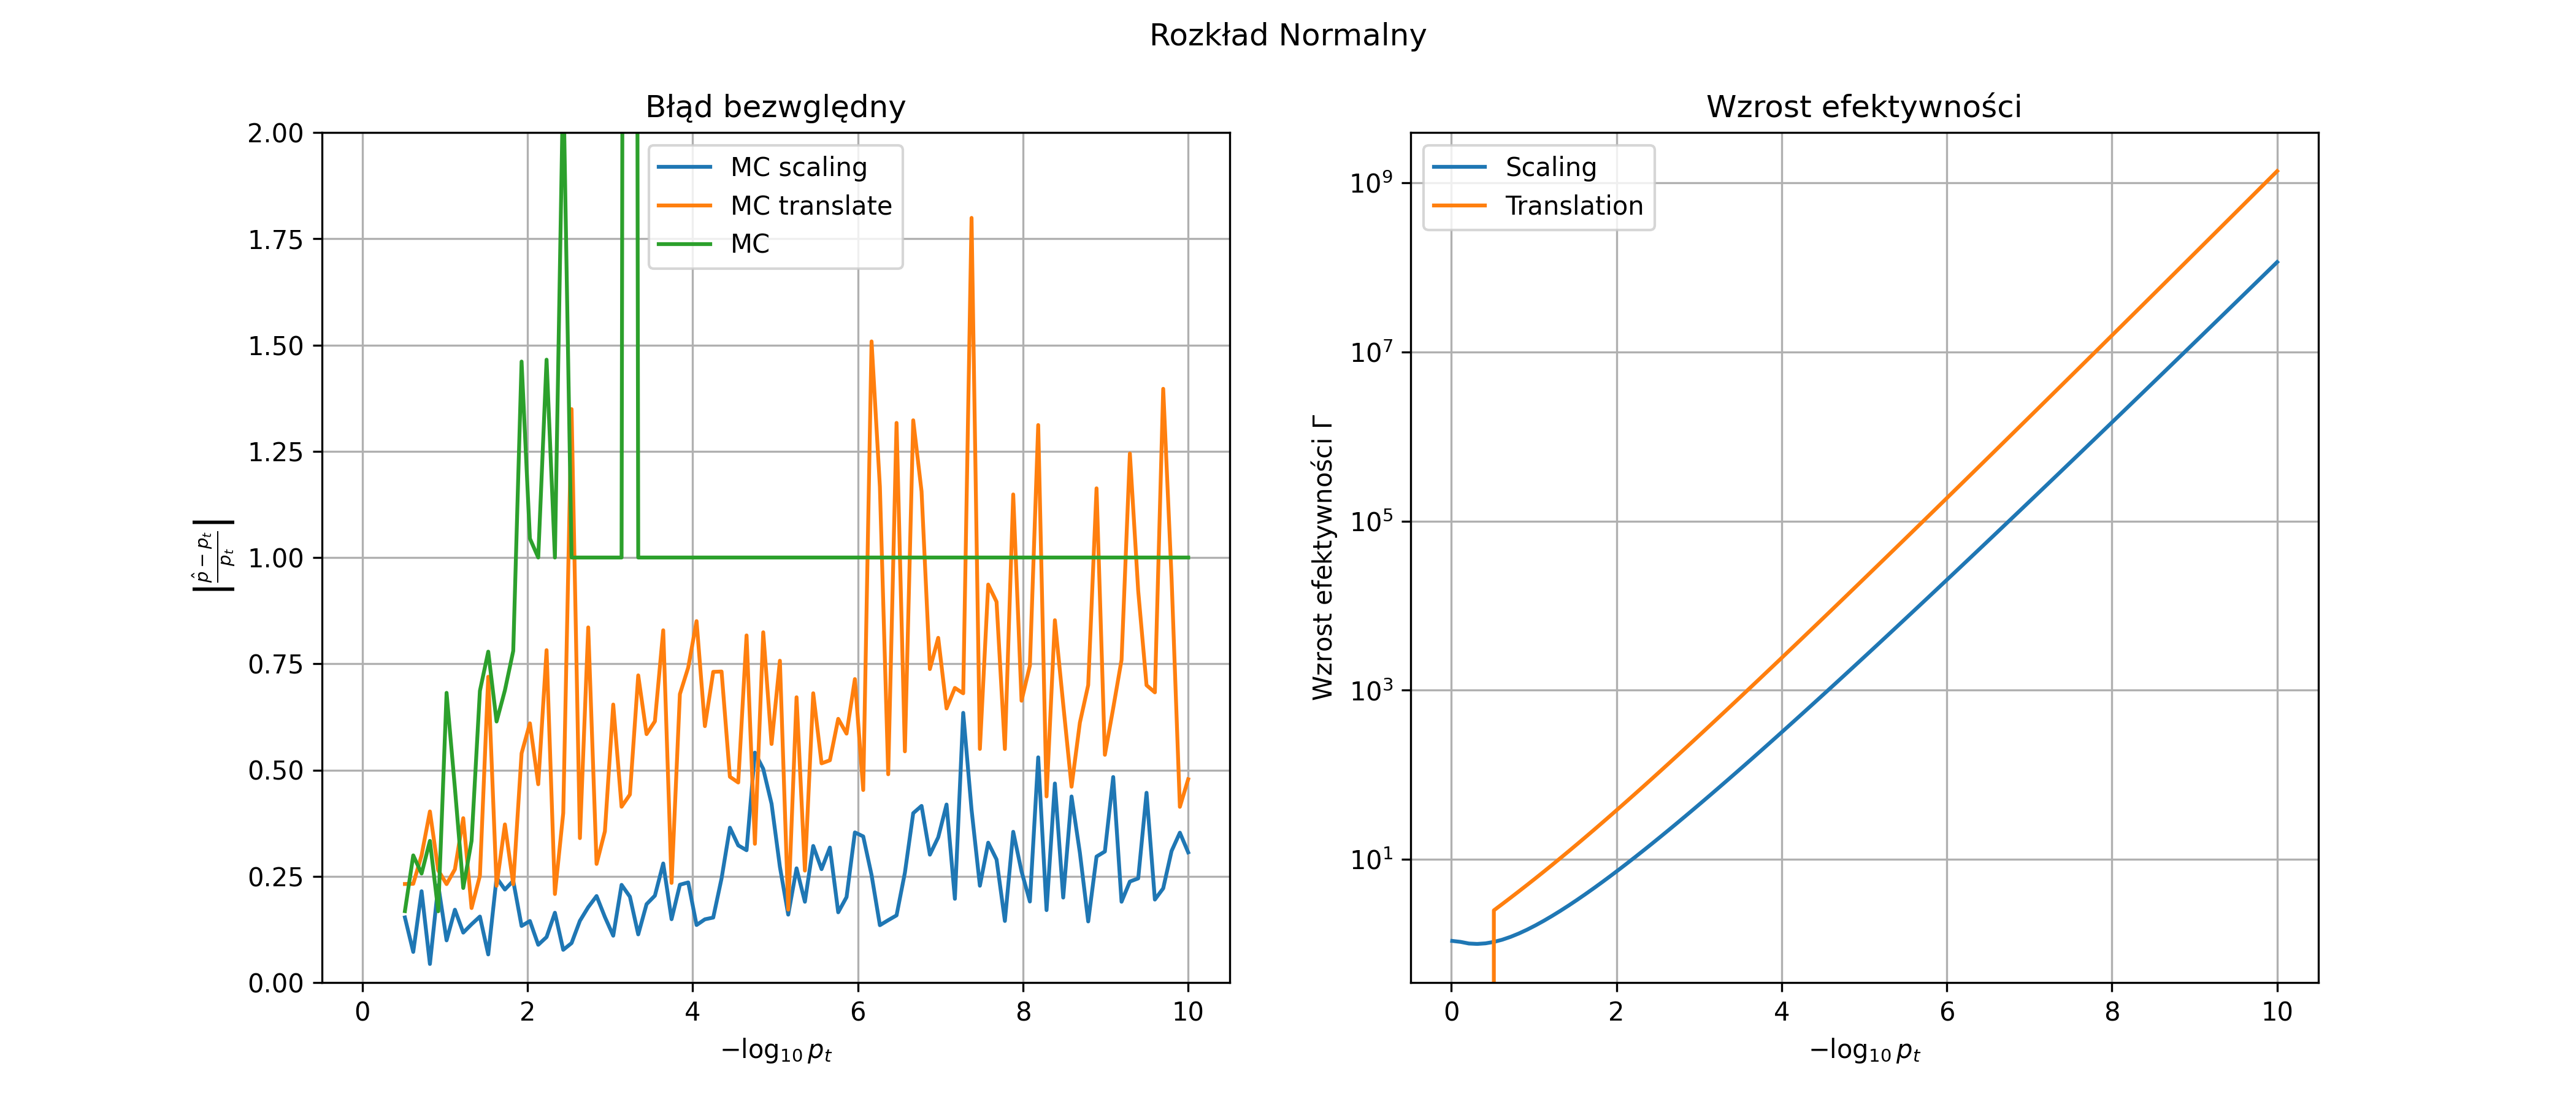
\includegraphics[width=\textwidth, height=\textheight, keepaspectratio]{nowe/subblots_normal.png} \end{figure} \end{frame}

\begin{frame}{Testowanie numeryczne}{Rozkład Weibull}\begin{figure} 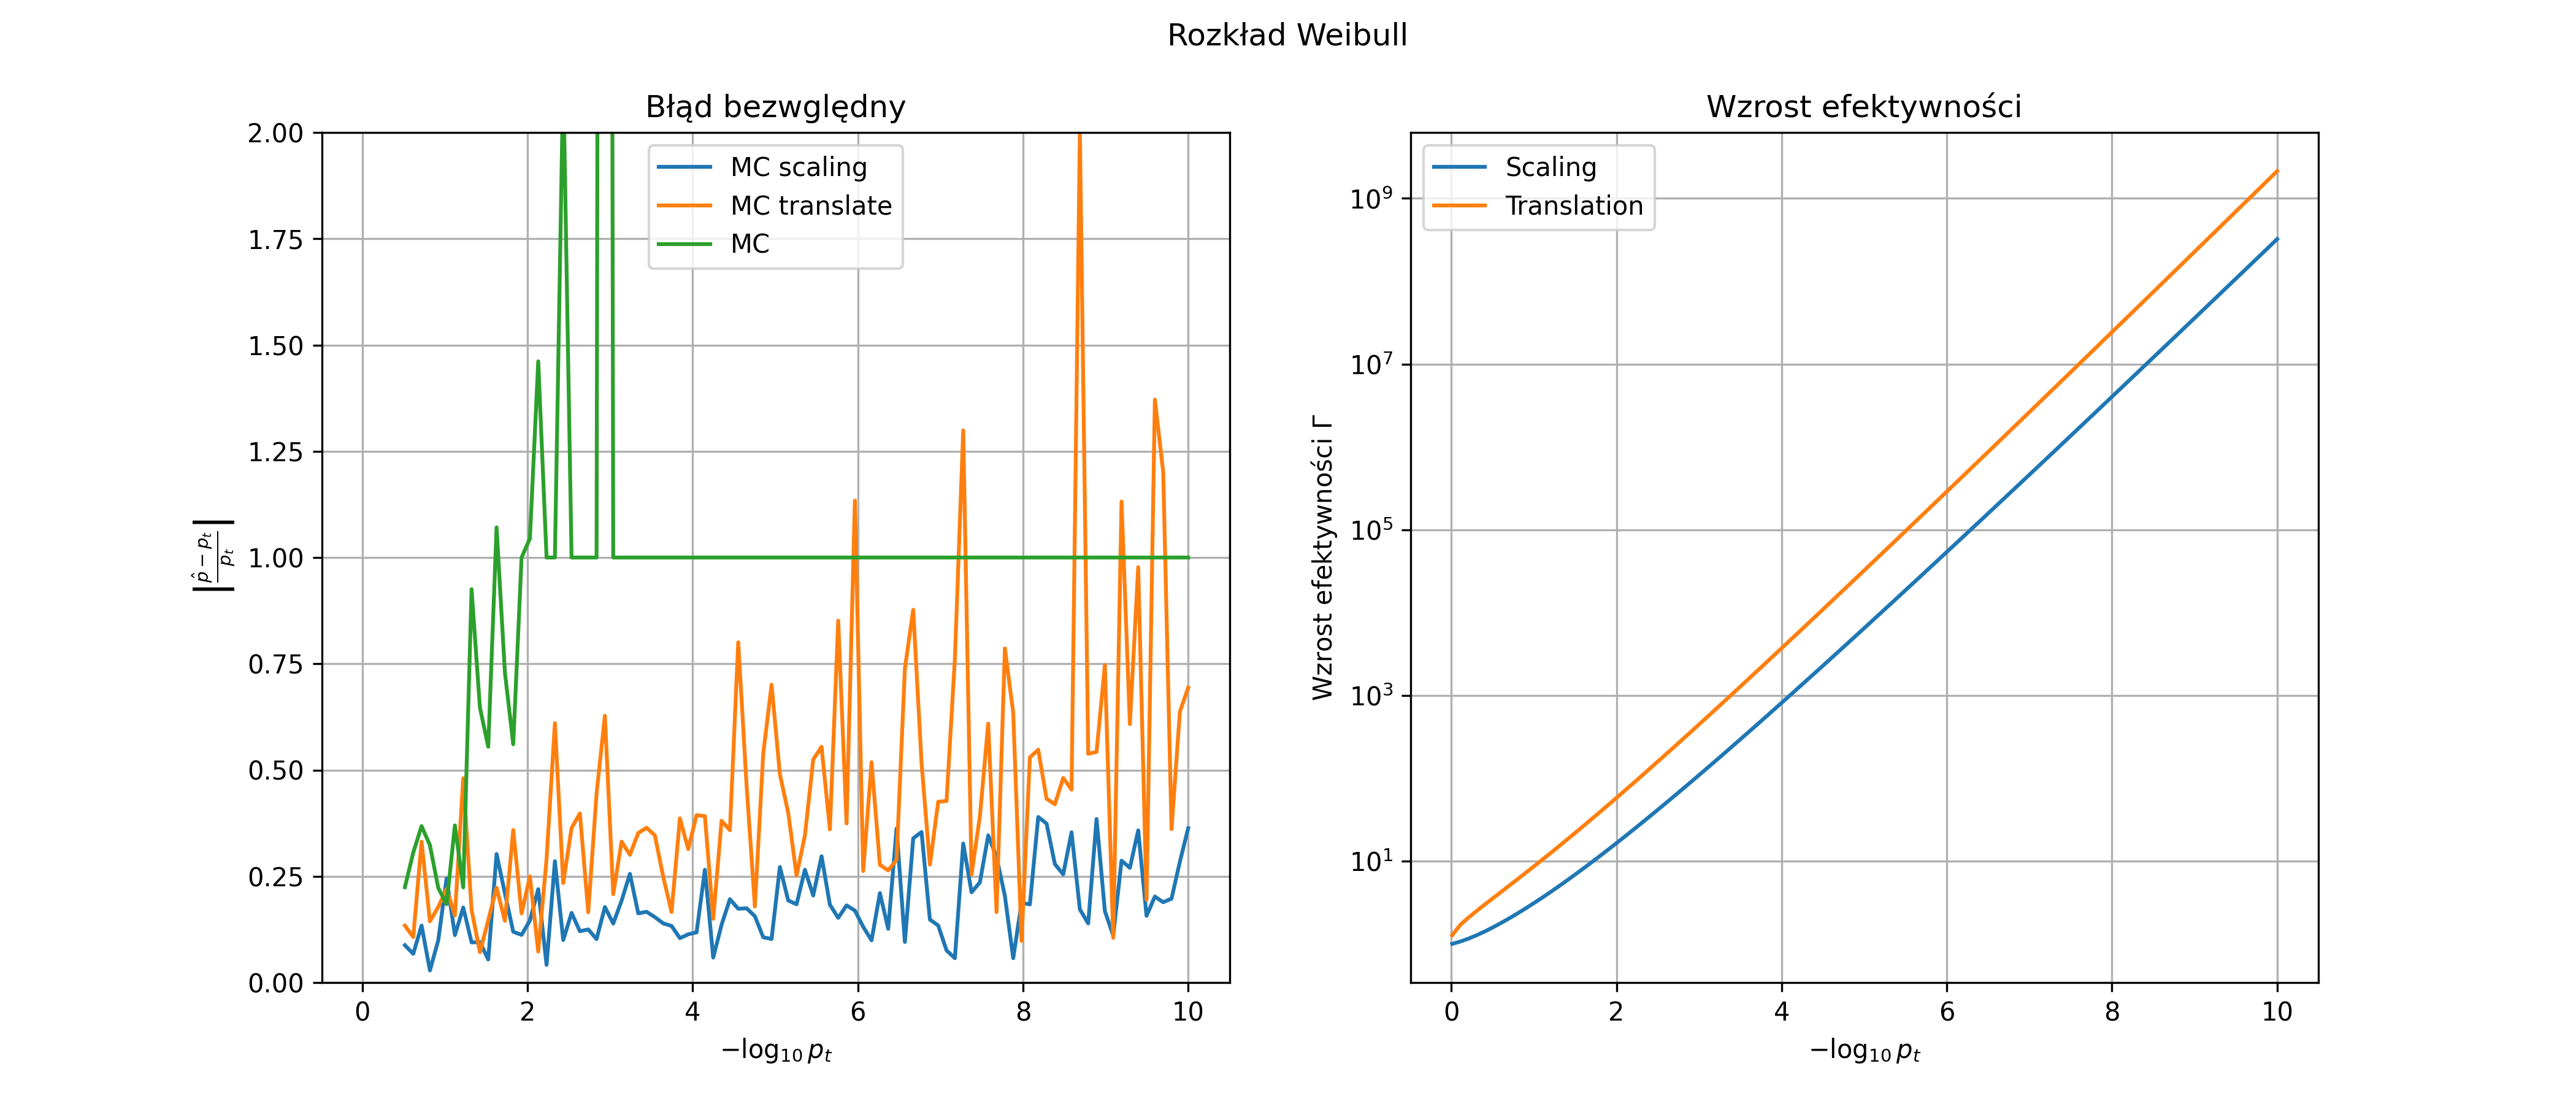
\includegraphics[width=\textwidth, height=\textheight, keepaspectratio]{nowe/subblots_weibull.png} \end{figure} \end{frame}
eeeew

\begin{frame}{Bibliografia}
 \bibliographystyle{apalike}
\nocite{*}
\bibliography{mybib} \end{frame}

\end{document}
